\chapter{Optimal Control}
\label{ch3}

%%%%%%%%%%%%%%%%%%%%%%%%%%%%%%%%%%%%%%%
% IMPORTANT
\singlespacing % THESE THREE
\minitoc % LINES MUST APPEAR IN
\doublespacing % EVERY CHAPTER
% COPY THEM IN ANY NEW CHAPTER
%%%%%%%%%%%%%%%%%%%%%%%%%%%%%%%%%%%%%%%

\section{Mean-Variance MPC Framework}

\subsection{Introduction to MPC}

\ac{MPC} is a control technique in which given a state space $X$ and control variables on the input space $U$ over a certain time horizon $T$, the control law selected is such that the objective function (that depends on the state and input values) is minimized/maximized subject to constraints over the horizon \cite{PredictiveControl}. After the control law is selected a certain number of control sequences are applied before repeating the procedure.

Moreover several optional modifications can be done to the controller to make it more adaptive to disturbances or  mismatches against the physical system, as well as to improve its computational efficiency over time by introducing  model parameter estimation or variable horizon functionalities in the loop, this can be done either before the optimization routine begins during "Pre-checks" or afterwards during "Post-checks", for example after the optimization routine ends if there are any constraint violations one could increase the sampling frequency, or given the current state one could decide to reduce the horizon. 

Figure \ref{fig::ch3_MPC} shows a diagram representing the MPC overall algorithm.

\begin{figure}[h!]
    \centering
    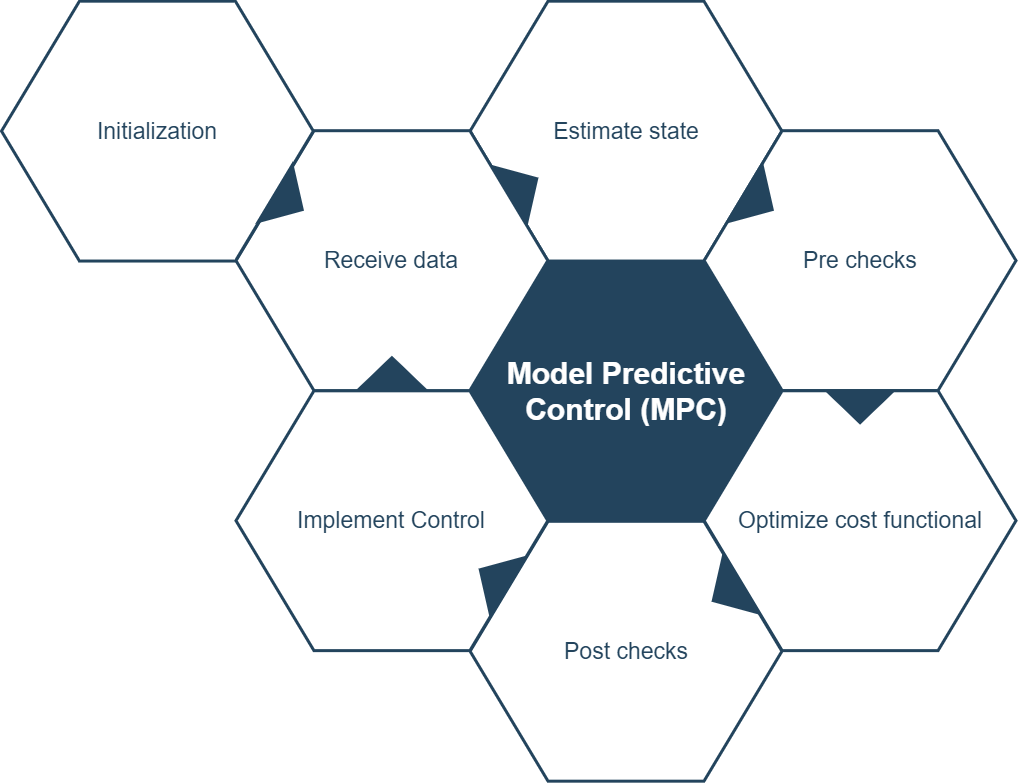
\includegraphics[width=1\textwidth]{imgs/ch3/MPC drawing.png}
    \caption[\ac{MPC} logic diagram]{\ac{MPC} logic diagram}
    \label{fig::ch3_MPC}
\end{figure}

In this section the elements of the model predictive control used in this project are introduced. With particular emphasis to its application in multi-period portfolio optimization. Many of elements of this formulation can be attributed to the paper published by Xiaoyue Li in 2022 \cite{MultiPeriod_PO_mpc}.

\subsection{Formulation}
This method tries to solve a \ac{LQP}  were the cost functional has a negative quadratic term for each daily(transition) variance day and a positive linear term for returns \cite{MultiPeriod_PO_mpc}. By minimizing such cost functional a trade-off between expected risk (variance) and expected returns is achieved, not in a ratio sense like optimizing Sharpe but in opposing forces of a \ac{LQP}  problem \cite{MultiPeriod_PO_mpc}. 

Letting $N$ be the number of assets considered for the optimization problem.

\textbf{State Space:} The vector of expected returns and the covariance matrix at each point in time, $\left[r_{t+1|t},...,r_{t+H|t}\right]$ and $\left[\Sigma_{t+1},...,\Sigma_{t+H}\right]$, where $r_i \in \R^N$ and $\Sigma_i \in \R^{N\times N}$, therefore the state space {T()}belong in $\R^{H \times N\times(N+1)}$.

\textbf{Input Space:} The control variable in this formulation is the allocation of assets with respect of the total value of the portfolio at each point in time, represented by $\left[\pi_{t+1},...,\pi_{t+H}\right]$.

\textbf{Objective Function:} A quadratic form (\ref{eq::c3_Objective}) to maximize the expected return given a quadratic cost in term of the uncertainty with a proportional cost on the transacted ratio.

\begin{equation} \label{eq::c3_Objective}
\max_{\pi_{t+1},...,\pi_{t+H}} \left(\sum_{\tau=t+1}^{\tau=t+H} \hat{r}^{T}_{\tau|t}\pi_{\tau} 
- \gamma^{risk}\left(\pi_{\tau}^T \hat{\Sigma}_{\tau|t}\pi_{\tau}\right) 
- \gamma^{trade}||\pi_{\tau}-\pi_{\tau-1}||_1
\right)
\end{equation}
The hyper-parameters of the objective function are $\gamma^{risk}$ the tisk aversion parameter and $\gamma^{trade}$ the transaction cost.


\textbf{Constraints:} The basic constraints in this problem are that all entries in allocation vector to be greater or equal than zero, which is equivalent to no edging (\ref{eq::ch3_noEdgingConstraint}), and that the sum of the allocation at any point in time adds up to 1 (\ref{eq::ch3_unitAllocationConstraint}).

\begin{equation}\label{eq::ch3_noEdgingConstraint}
\pi_{\tau}\geq 0\quad \forall\tau=t+1,...,t+H
\end{equation}

\begin{equation}\label{eq::ch3_unitAllocationConstraint}
\textbf{1}^T\pi_{\tau}=1 \quad \forall\tau=t+1,...,t+H
\end{equation}

Also it is possible to place constraints on the returns at any point in time (\ref{eq::ch3_iReturnConstraint}), or forbid holding shaeres of a particular company ``$j$" assets at time $\tau$ (\ref{eq::ch3_forbidAssrtConstraint}).

\begin{equation}\label{eq::ch3_iReturnConstraint}
 \hat{r}^{T}_{\tau|t} \pi_{\tau} - \text{minVal} \geq 0
\end{equation}

\begin{equation}\label{eq::ch3_forbidAssrtConstraint}
  \pi_{\tau,j} = 0 
\end{equation}


Or by assuming the returns distribution in each time to be independent from each other, one can use the overall expected return between time $t$ and $i$ at $t$ (\ref{eq::ch3_overallReturn}) to define more complex constraints such as ``minimal accumulated expected return at time i" (\ref{eq::ch3_iAccumReturnConstraint})
``Minimum portfolio value"(\ref{eq::ch3_iMinPortfolioConstraint}).


\begin{equation}\label{eq::ch3_overallReturn}
    \hat{r}_{[t,i|t]}=\prod_{\tau=t+1}^{i} \hat{r}^{T}_{\tau|t}\pi_{\tau} - \gamma^{trade}||\pi_{\tau}-\pi_{\tau-1}||_1 
\end{equation}

\begin{equation}\label{eq::ch3_iAccumReturnConstraint}
    \hat{r}_{[t,i|t]} - \text{minVal} \geq 0
\end{equation}


\begin{equation}\label{eq::ch3_iMinPortfolioConstraint}
   \text{initialCapital} \hat{r}_{[t,i|t]} - \text{minPortfolioVal} \geq 0
\end{equation}

Finally constraints such as initial capital amount, are implemented as parameters of the MPC whilst the control variable operates on portfolio scaled by the initial capital. 

\textbf{System dynamics:}
In order to estimate the dollar value of the composition of the portfolio over future periods of time it is necessary to be able to estimate the value of different assets over time or more precisely the expected period return. This is done through forecasting.

\subsection{Forecasting}

In this section the forecasting/estimation of the return vector and covariance matrices is addressed, first a brief discussion on causality between measurable attribute and asset prices will be carried out, followed by descriptions of several forecasting methods used in the experiments on Chapter \ref{ch5}.

It is important to notice that a necessary condition for the objective function (\ref{eq::c3_Objective}) to output sensible input sequences when optimized is for the covariance matrices to be positive definite. Some of the methods do not guarantee such result, for those methods the objective function (\ref{eq::c3_Objective}) is modified to not include the quadratic terms.

\subsubsection{Discussions on causality}
Before proceeding into the specifics of the model is worth studying the potential causality between attributes of assets, either causal relationship between assets, that can come in different shapes. Since the nature of the model in the model-free formulation won't be guessed the factors to be taken into account for the model should have some degree of relationship between each other in order to make more useful control systems, meaning to have a model capable of better predictions when considering the effect of controllable variables and other state variables.

\begin{enumerate}
    \item Do poor performance of agricultural companies have a domino effect on the performance of other companies in the Food industry or fashion industry and can this be observed through the stock price?
    \item Can changes in the price and traded volume may affect each other, therefore can there be a bi-directional causality may exist as in a closed loop system?
    \item Can broad macro-economic factors influence the overall direction of stock prices?
    \item Can regulatory reforms impact the dynamics between attributes with causal relationships?
    \begin{enumerate}
        \item What about market structures such like monopolies and cartels? 
        \item Under what conditions can we assume causal relationships can be maintained? 
        \item How fast the algorithms need to be in order to adapt to unobservable events as regulatory or market power changes, meaning how long into the past a human observer need to be aware of changes that can affect the thrust-worthiness of the output of the model?
    \end{enumerate}
\end{enumerate}   

\textbf{Price-Volume causality:} Price volume causality is a widely studied subject with mixed results and no clear general answer, from an abstract point of view for each sale that happens there must have been a purchase, therefore the amount of sales and its price don't need to be related however at closer inspection under particular circumstances there may be evidence of the contrary. 

There are individual pieces of evidence that suggest a causal relationship between price and volume as in the case of the GameStop frenzy were the timing of the selling and buying of shares of GameStop forced the price to go up and forced many short-sellers to liquidate their positions in a distressed sale \cite{game_stop_case}. Although this example is a form of predatory trading that carries with it a deep ethical discussion it does show that is possible to affect price with volume and likely vice versa, at least under particular circumstances.

A study in the stock exchange in India suggest by using Granger causality suggest that the causality between volume traded and price fluctuate over time depending on market reforms and presence of feedback trading between 95'and 21' having price driving volume and after 21' no relation \cite{price_volume_causality_india06}.

A more recent study suggest that the Granger test for linear causality and its extension by Hiemstra and Jones for nonlinear Granger causality is prone to over-rejection by using Monte Carlo simulations and introduced a model free test based on conditional permutation-entropy to measure nonlinear causality. This method was applied to the SP500 between 1950 and 1990 and it suggested the existence of a causal relationship between price and volume both on mean and variance for daily trade \cite{price_volume_causality_enthropy}.

\subsubsection{Behavioural forecasting}
This method is a modified version of the \ac{DeePC}\cite{og_deepc}, which is arises from an application of the fundamental lemma of behavioural systems \cite{precursor_deepc,fundamentalLemma}. Is worth noticing that in its application one of the hypothesis has been relaxed in particular the one of the controllability of the system.

The fundamental lemma states that for a \ac{LTI} controllable system any trajectory in the input-output space can be expressed as a linear combination of past trajectories \cite{fundamentalLemma}. Lets consider the Hankel matrix (\ref{eq::hankelMatrix}) of an autonomous system with output $y$ which at time t takes the value $y_t$, this matrix on each column contains trajectories of length $N$. 

\begin{equation}
    \label{eq::hankelMatrix}
    H(y)= \begin{bmatrix}
y_1 & \cdots & y_{t-N+1}\\
\vdots & \ddots & \vdots\\
y_N & \cdots & y_t
\end{bmatrix}
\end{equation}

Now consider two integers $p$ and $f$ such that $p+f=N$ and $p\geq1$, $f\geq1$, termed past and future windows. Lets also split the Hankel matrix into the past and future Hankel submatrices (\ref{eq::hankelMatrixpf}). Furthermore, consider that we have knowledge of the past $p$ values of the output $y$, the trajectory of the past $p$ values can be determined as a linear combination of the columns of $H_p(y)$ such that $g=H_p(y)\backslash  y_{t-p+1:t}$. the behavioural forecasting predicts the following $f$ values of $y$ as the linear combination of $\hat{y}_{t+1:t+f} = H_f(y)*g$ 

\begin{equation}
    \label{eq::hankelMatrixpf}
    H(y)= \begin{bmatrix}
y_1 & \cdots & y_{t-N+1}\\
\vdots & \ddots & \vdots\\
y_p & \cdots & y_{t-p+1} \\
y_{p+1} & \cdots & y_{t-p+2} \\
\vdots & \ddots & \vdots\\
y_N & \cdots & y_t
\end{bmatrix}\Rightarrow{} \quad 
\begin{array}{l}
H_p(y)= \begin{bmatrix}
y_1 & \cdots & y_{t-N+1}\\
\vdots & \ddots & \vdots\\
y_p & \cdots & y_{t-p+1} 
\end{bmatrix}\\
 H_f(y)= \begin{bmatrix}
y_{p+1} & \cdots & y_{t-p+2} \\
\vdots & \ddots & \vdots\\
y_N & \cdots & y_t
\end{bmatrix}
\end{array}
\end{equation}

\subsubsection{Hidden Markov Model (\ac{HMM})}

\ac{HMM} is a method that predicts the expected return vector and the covariance matrix to be in a discrete set of states that are not directly observable, each state is represented as a time-invariant stochastic process were at each time-instant the returns follow a  Multivariate Gaussian distribution with fix mean vector and covariance matrix \cite{MultiPeriod_PO_mpc}.

Given past data, the Baum-Welch method \cite{OG_BaumWelch} is used to estimate the transition probability between these hidden states and the coefficients of the MultiVariate Gaussians associated to each hidden state.

Using recent past data the current state is estimated, and the forecast of covariance and mean vectors is computed in an iterative manner, is worth pointing out that at the moment the ``HiddenMarkovModels.jl" package \cite{HiddenMarkovModels.jl} in Julia just estimates the most likely state, and it doesn't provide the most likely probability distribution of states, which could be used for a refinement of the forecast vectors and matrices.

A huge advantage of this method is that if the coefficients of the HMM are not modified significantly the forecast matrices will only depend on the current state, and it can be precomputed and save in memory.

Following the work of Guidolin \cite{numberOfRegimes} two states known as ``bull" and ``bear" (or ``normal" and ``contraction") shall be used in the \ac{HMM}, . Thus the transition matrix between the states (\ref{eq::ch3_HMM_TransitionMatrix}) is a $2\times2$ matrix where $p_{nn}$ is the probability of remaining in the normal regime, whilst $p_{cc}$ is the probability of remaining on the contraction regime following the notation of Li \cite{MultiPeriod_PO_mpc}.

\begin{equation} \label{eq::ch3_HMM_TransitionMatrix}
    T_{hmm}=\begin{bmatrix}
        p_{nn} & 1- p_{nn} \\
        1-p_{nn} & p_{cc} \\
    \end{bmatrix}
\end{equation}

During the normal regime the model assumes the returns to follow a distribution $\D_n=\Normal{n}$ and during the contraction regime $\D_c=\Normal{c}$. 

\textbf{Forecast algorithm:} Let $q_t=[q_{t,n},q_{t,c}]$ be the probability distribution of the state at time t the forecast algorithm follows Algorithm \ref{algo::HMMForecast} which can be implemented in Julia by adapting Listing \ref{lst:HMMForecast}.

\begin{algorithm} \label{algo::HMMForecast}
    \caption{\ac{HMM} Forecast}
  \begin{algorithmic}[1]
  \Require Determine $q_0,\quad \Normal{n},\quad\Normal{c}$
  \State $V_\mu = \begin{bmatrix} \mu_n \\ \mu_c\end{bmatrix}$   
  \State $V_\Sigma = \begin{bmatrix} \Sigma_n \\ \Sigma_c\end{bmatrix}$   
  \State $\mu_0 = q_0'*V_\mu$
  \State $\Sigma_0 = q_0'*V_\Sigma$ 
    \For{\texttt{i=0:Horizon-1}}
        \State $q_{i+1} = T_{hmm}*q_i$ 
        \State $\mu_{i+1} = q_{i+1}*V_\mu$
        \State $\Sigma_{i+1} = q_{i+1}*(V_\mu + \begin{bmatrix}
           (\mu_n-\mu_{i+1})*((\mu_n-\mu_{i+1})') \\
           (\mu_c-\mu_{i+1})*((\mu_c-\mu_{i+1})')
        \end{bmatrix}$
    \EndFor
  \end{algorithmic}
\end{algorithm}


\begin{lstlisting}[language=Julia,escapeinside={(*}{*)},label={lst:HMMForecast},caption={Example implementation of HMM Forecast in Julia},captionpos=b]
# The following is a Pseudo-code, not intended to be executed alone
    using HiddenMarkovModels
    hmm=...; # Hidden Markov Model variable
    N=length(hmm); # Number of states
    fitDists=[obs_distribution(hmm,i) for i=1:length(hmm)]; # Distributions of each state
    (*V\mu*)= [f.(*\mu*) for f=fitDists]
    (*V\Sigma*)=[f.(*\Sigma*) for f=fitDists]
    q0 = zeros(N);
    q0[get_current_state(hmm,context.extra.obs_seq)] = 1 # Probability of each state at t=0
    (*\mu*)0 = sum(q0.*(*V\mu*)); (*\Sigma*)0 = sum([ q0[i].*(*V\Sigma*)[i] for i=1:N])
    M=length((*\mu*)0) 
    # Pre-allocation of output
    forecast = [(zeros(M),zeros(M,M)) for i=1:futureHorizon] 
    for i=1:futureHorizon
        q1 = transition_matrix(hmm)*q0
        (*\mu*)1 = sum(q1.*(*V\mu*))
        (*\Sigma*)1 = sum([ q1[i].*((*V\Sigma*)[i] + (((*V\mu*)[i]-(*\mu*)1)*((*V\mu*)[i]-(*\mu*)1)'))  for i=1:N]) 
        q0,(*\mu*)0,(*\Sigma*)0=q1,(*\mu*)1,(*\Sigma*)1
        forecast[i][1][1:M]=(*\mu*)1
        forecast[i][2][1:M,1:M]=(*\Sigma*)1
    end
\end{lstlisting}

\subsubsection{Benchmarks}
In order to benchmark the Behavioural and \ac{HMM} methods two basic but well established forecasting techniques will be used as a comparison.

\textbf{Linear regression:} In this method the expected return of each asset over with sample window ``$w_s$" is adjusted through a linear regression over a sample of length $w_{lr}$, this produces an estimate on the expected return vector. 

Is worth pointing out that the same technique cannot be used for the covariance matrix,at least on a per entry level because the matrix is not guaranteed to be positive semi-definite.

\textbf{Last value:} This is the forecasting technique used by the Markowitz strategy, in this technique the future return matrix and covariance matrix is expected to be the same as in the immediate past data over a sample window of individual asset returns ``$w_s$" which can be different for the estimation of expected returns $w_{s\mu}$ and the covariance matrix $w_{s\Sigma}$. 
